\begin{figure*}%[!htbp]
\begin{center}


\begin{subfigure}[b]{0.95\columnwidth}
  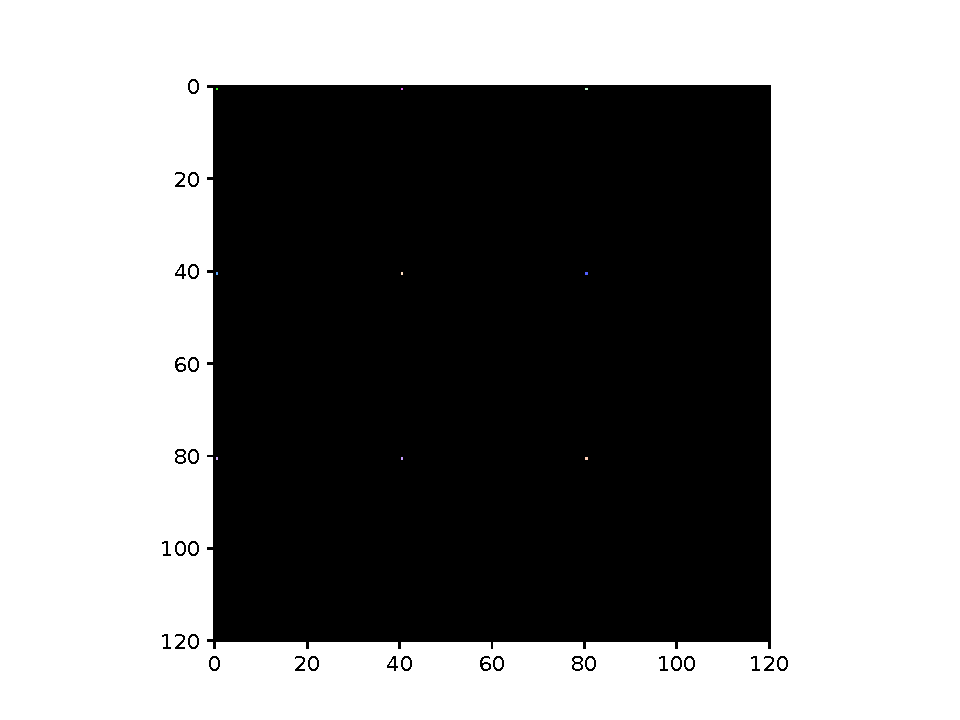
\includegraphics[width=\columnwidth,trim={2.5cm 0.5cm 2.5cm 1cm},clip]{img/ChannelMap_1030_update0}
  \vspace{-5ex}
  \caption{Update 0; cell gen. 0}
  \label{fig:ChannelMap_1030_update0}
\end{subfigure}%
\begin{subfigure}[b]{0.95\columnwidth}
  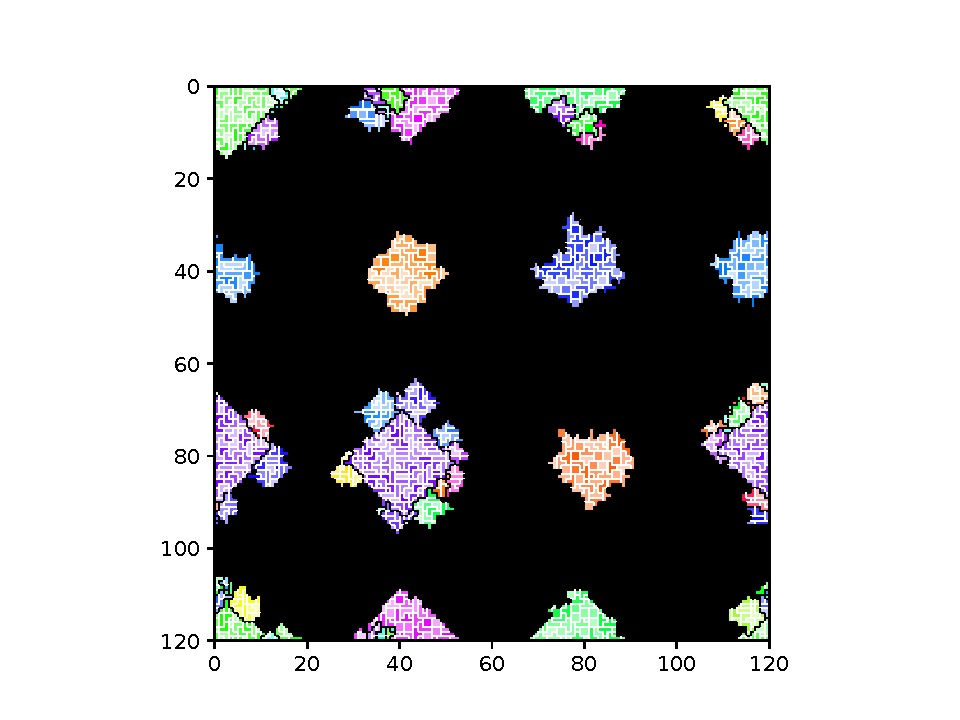
\includegraphics[width=\columnwidth,trim={2.5cm 0.5cm 2.5cm 1cm},clip]{img/ChannelMap_1030_update5552}
  \vspace{-5ex}
  \caption{Update 5552; cell gen. 4}
  \label{fig:ChannelMap_1030_update55520}
\end{subfigure}

\begin{subfigure}[b]{0.95\columnwidth}
  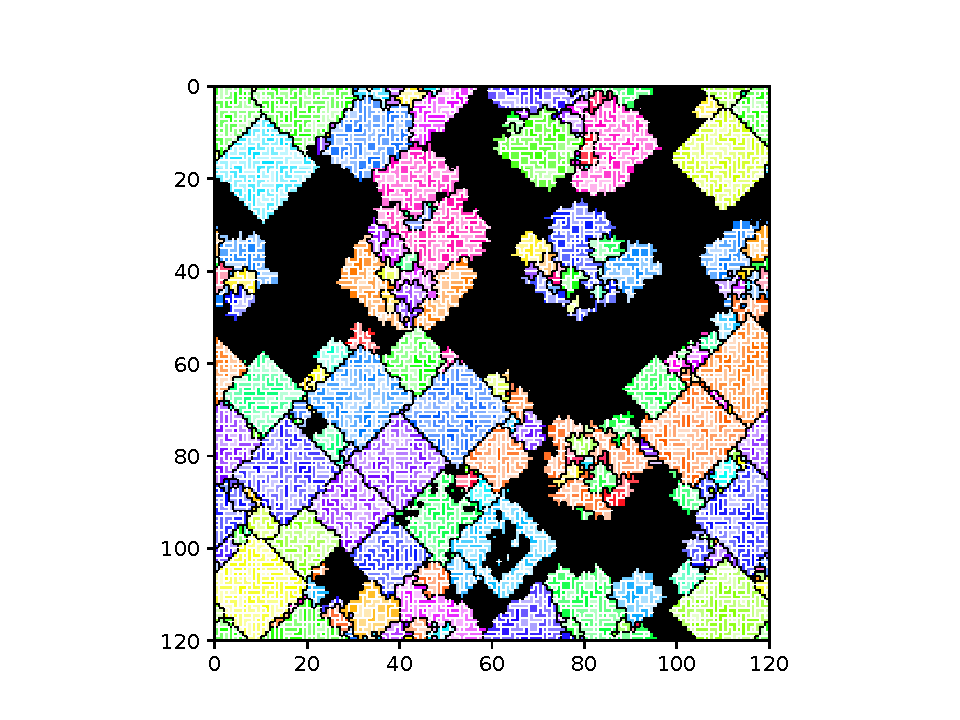
\includegraphics[width=\columnwidth,trim={2.5cm 0.5cm 2.5cm 1cm},clip]{img/ChannelMap_1030_update11104}
  \vspace{-5ex}
  \caption{Update 1104; cell gen. 9}
  \label{fig:ChannelMap_1030_update277600}
\end{subfigure}%
\begin{subfigure}[b]{0.95\columnwidth}
  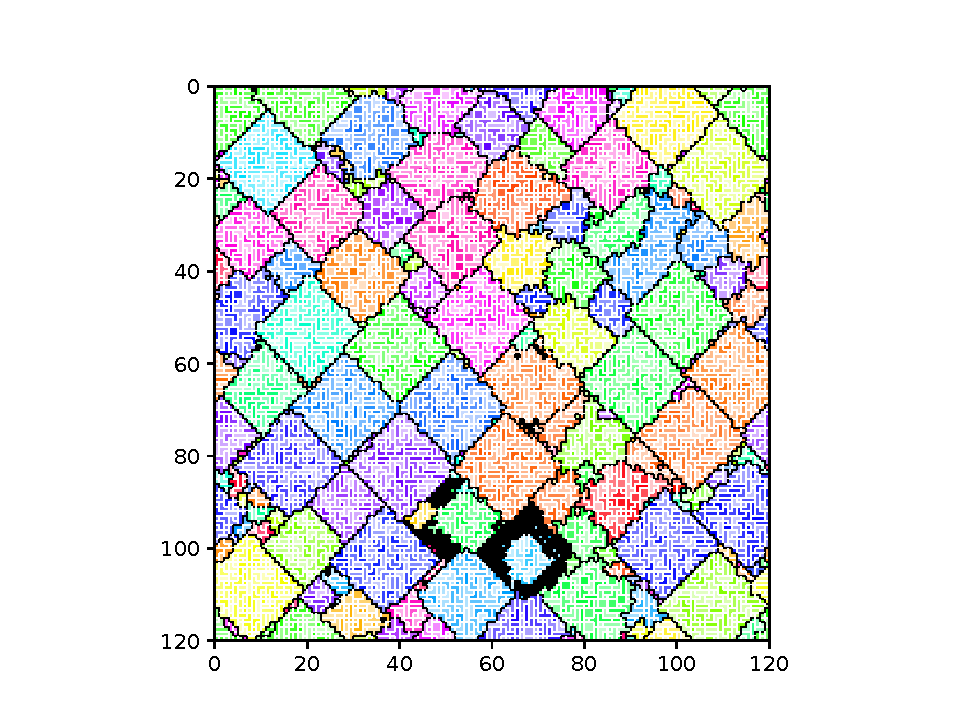
\includegraphics[width=\columnwidth,trim={2.5cm 0.5cm 2.5cm 1cm},clip]{img/ChannelMap_1030_update22208}
  \vspace{-5ex}
  \caption{Update 22208; cell gen. 32}
  \label{fig:ChannelMap_1030_update22208}
\end{subfigure}

\begin{subfigure}[b]{0.95\columnwidth}
  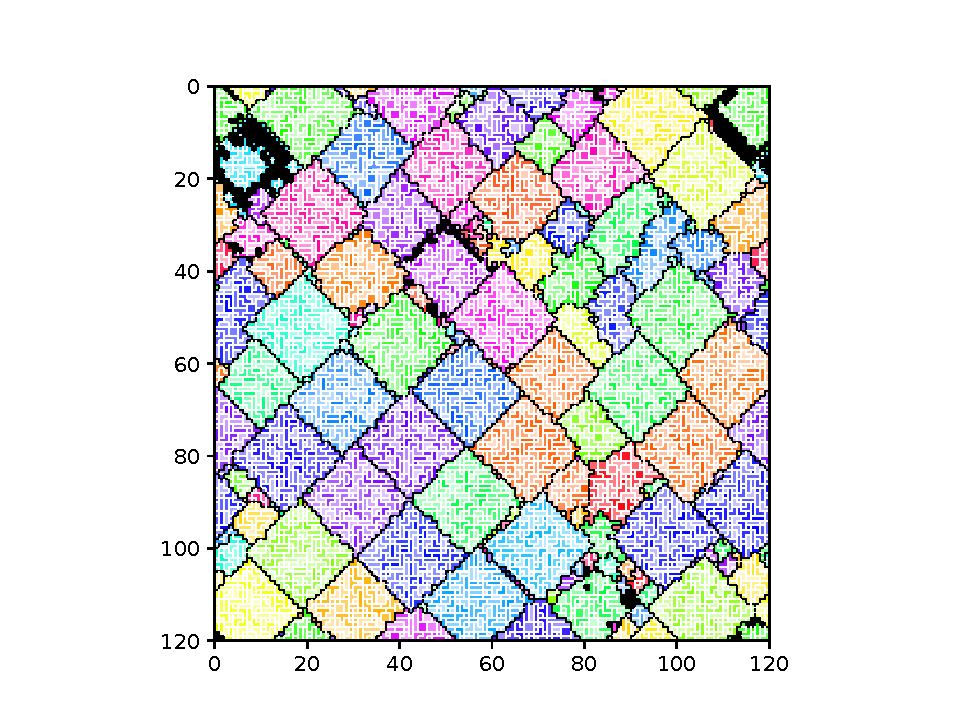
\includegraphics[width=\columnwidth,trim={2.5cm 0.5cm 2.5cm 1cm},clip]{img/ChannelMap_1030_update55520}
  \vspace{-5ex}
  \caption{Update 55520; cell gen. 107}
  \label{fig:ChannelMap_1030_update1000000}
\end{subfigure}%
\begin{subfigure}[b]{0.95\columnwidth}
  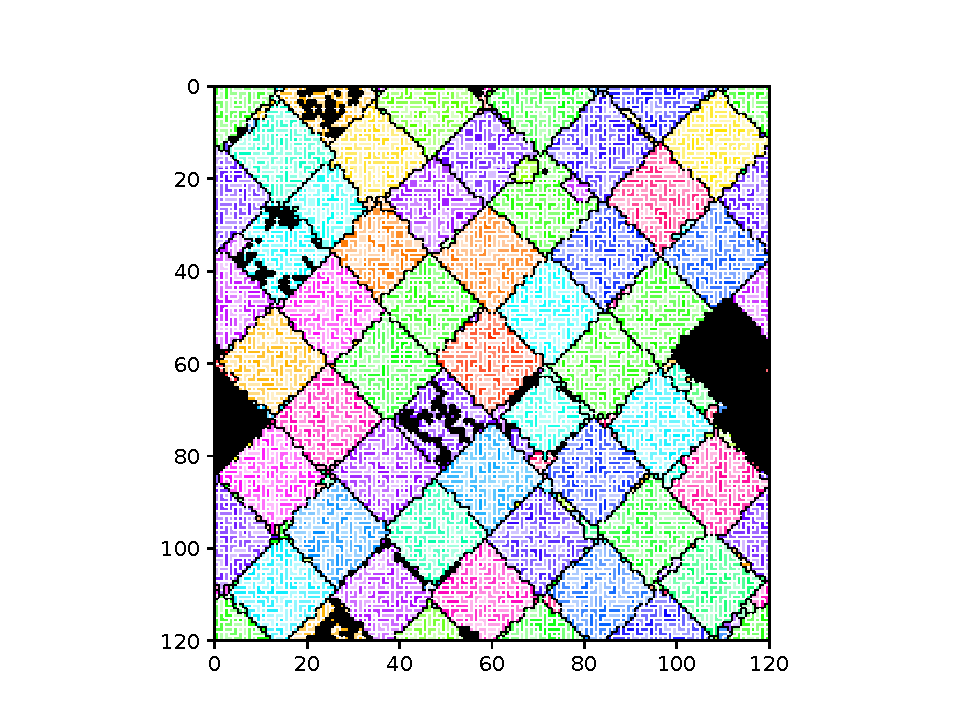
\includegraphics[width=\columnwidth,trim={2.5cm 0.5cm 2.5cm 1cm},clip]{img/ChannelMap_1030_update1500000}
  \vspace{-5ex}
  \caption{Update 1500000; cell gen. 3511}
  \label{fig:ChannelMap_1030_update1500000}
\end{subfigure}
\caption{
Progression of of same-channel level-one and level-two signaling networks states in a competition run.
We seeded the grid with three copies of each of three champion genotypes from evolutionary trials.
Then, with mutation disabled to prevent further evolution, the genotypes competed.
Level-one channels are coded by color saturation and level-two channels are coded by color hue.
A single cell-like organism occupies each grid tile except for black tiles, which are empty.
}
\label{fig:eco_progression}
\end{center}
\end{figure*}
